%% ------------------------------------------------------------------------- %%
\chapter{Introdução}
\label{cap:introducao}


A durabilidade e vida útil do cimento tem sido o problema mais importante enfrentado pela indústria de construção civil nas últimas décadas \citep{cementml}. Os custos de manutenção são da ordem de bilhões de dólares e portanto, a capacidade da previsão de propriedades do cimento desde a sua produção ganha grande importância. Une-se a isso a presença cada vez maior de métodos de ML em domínios diversos da engenharia e ciência e surge então a tentativa de usar algoritmos de aprendizado também para esse domínio (\cite{cementnn1}, \cite{cementnn2}). \\ 

Esse trabalho é uma colaboração entre a empresa Intercement e o Laboratório de
Lógica, Inteligência Artificial e Métodos Formais do IME-USP. Foram concedidos
10 anos de dados de diversas etapas da produção de cimento do complexo de
Cajati, uma das plantas da empresa. Esse trabalho é um estudo com a análise
desses dados, desde o seu pré-processamento até uma criação de modelos
preditivos e a investigação de sua acurácia. \\


Os dados são medições de diversos parâmetros em meio ao processo de fabricação do cimento. Eles são divididos em diversas planilhas para diferentes etapas da produção de cimento, são elas, em ordem no processo:

\begin{itemize}
        \item Cimento Cru
        \item Farinha
        \item Clinquér
        \item Produção de Cimento
        \item Expedição de Cimento
\end{itemize}


Esse trabalho irá aplicar métodos modernos de ML e DP para a modelagem desses
dados. Dado que o problema em questão é de \textbf{regressão}, i.e. queremos
prever valores numéricos, saímos do domínio canônico onde são aplicados métodos
de DL, como por por exemplo processamento de linguagem natural ou visão computacional. Nesse trabalho serão estudados modelos propostos por \citet{ubertime} e \citet{energylstm} para problemas de regressão.

\section {Motivação}

Esse trabalho tenta ir além de publicações recentes do próprio domínio de Engenharia Civil como \cite{cementnn1},
\cite{cementnn2} e \cite{cementml}, usando métodos de DL que tem
obtido excelentes resultados em tarefas de
regressão com dados sequenciais, não necessariamente de produção de cimento. Esse trabalho irá reproduzir modelos
propostos em \cite{ubertime}, \cite{energylstm}, \cite{deepar} e \cite{deepfactors} em que
técnicas de DL são usadas para modelagem de dados de demanda de carros e de energia elétrica. 

Como comparação e \textit{baseline} iremos comparar os resultados com uma regressão linear dinâmica como proposto por \cite{greciaLin},
no próprio domínio da produção de cimento.

%% ------------------------------------------------------------------------- %%
\section{Produção de Cimento}
\label{sec:producao}

Nessa seção será feito um breve resumo da produção de cimento, usando como base a figura a seguir: \\ 

\begin{figure}[H]
\centering
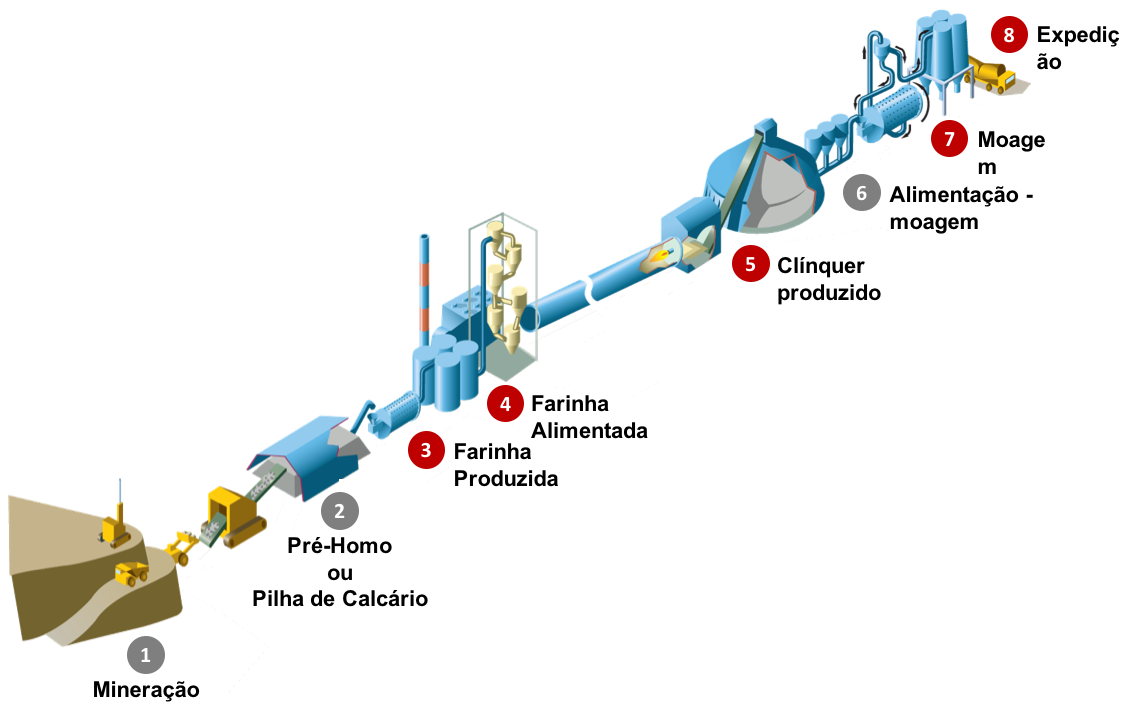
\includegraphics[width=0.9\columnwidth]{cimento.png}
\caption{Representação das Diversas Etapas da produção de Cimento \citep{cementroadmap}}
\end{figure}


As etapas de produção serão explicadas por número como indicado na imagem: \\

\begin{itemize}

\item[1] Depósitos ricos em carbonato de cálcio são mineirados para extração desse químico. Normalmente a planta é próxima da mina.
\item[2] O material extraido é triturado em pedaços de até 10cm. Diferentes materiais são misturados ao resultado da tritura, de modo a manter a composição química desejada. 
\item[3] A farinha crua é pré-aquecida para que depois no forno as reações químicas aconteçam mais rápido. 
\item[4] O cálcio é transformado em CaO por meio de reações químicas.  
\item[5] O material é introduzido ao forno, atingindo temperaturas de até $1450^\circ$C, transformando a farinha em clínquer. O clínquer é resfriado após a saída do forno. 
\item[6] O clínquer então é misturado com outros componentes que formam o cimento.
\item[7] A mistura é então moída.
\item[8] O material é empacotado, estocado e eventualmente expedido para entrega.

\end{itemize}

\subsection{Índice de Resistência de Cimento Portland}

A propriedade que iremos tentar prever usando nossos modelos será a resistência
compressiva do cimento. A resistência de uma amostra de cimento é ensaiada em
intervalos determinados de dias após a sua confecção. Essas informações são
anotadas nos dados com os nomes de $RCX$, com $X$ sendo a idade da amostra em
dias. Esses índices possuem a únidade de kPa, i.e. quilopascal.

%% ------------------------------------------------------------------------- %%
\section{Objetivos}
\label{sec:objetivo}

Gostariamos no desenvolvimento desse trabalho de obter resultados com a
aplicação de técnicas de DL recentes para um domínio inédito. Dessa maneira
abrindo portas para uma presença de aprendizado estatístico no processo de
engenharia da produção de cimento.


%% ------------------------------------------------------------------------- %%
\section{Organização do Trabalho}
\label{sec:organizacao_trabalho}

No Capítulo~\ref{cap:conceitos}, apresentamos os conceitos de Aprendizado de
Máquina, estatística frequentista e bayesiana, além de uma breve explicação
de cada modelo usado. No Capítulo~\ref{cap:estudodados} é mostrado de que
maneiras os dados foram tradados e modificados para facilidade de sua modelagem.
No Capítulo~\ref{cap:resultados} constam os resultados dos ensaios feitos com os dados. 



%%% Local Variables:
%%% mode: latex
%%% TeX-master: "../quali"
%%% End: